\section{Evaluation}\label{sec_evaluation}
In this section, we evaluate our proposed hybrid PSO algorithms for the allocation of software applications on heterogenous computing units, which conform to the system model presented in Section \ref{sec_system}. The algorithms are evaluated against different specifications of automotive software applications and execution platforms with regard to effectiveness, stabilitity and scalability. The software-application specifications consist of the number of software components $c$, runnables $r$, tasks $t$ and cause-effect chains $g$.  The specifications are synthesized from the automotive benchmark proposed by Kramel et al.~\cite{Kramer2015RealFree}. The benchmark indicates a strong correlation between runnables and cause-effect chains in terms of timing and activation patterns. It shows the timing specifications of runnables and their shares in an engine management system. Moreover, it shows the activation patterns of cause-effect chains, the runnables per activation and their shares in the system. The engine management system is one of the most complex automotive systems in the vehicular electical/electronic execution platform. 

\paragraph{Software Applications Benchmark} Based on our experience in the automotive industry, the benchmark results  are extrapolated to characterize different classes of automotive software applications specifications, that is by varying the parameters related to the software components, runnables, and cause-effect chains. The different classes of specifications range from Spec-I to Spec-V as shown in Table~\ref{tbl_appsspec}. The specification classes are useful to evaluate and discusse the effectiveness and scalability of the different optimization algorithms. The first specification class Spec-I encompases small software applications with number of components less than 10, runnables less than 50, tasks 30, cause-effect chains less than 30. The Spec-I and Spec-II classes represent medium and large software applications, and the last specification class is introduced to strech the performance analysis. 
\begin{table}
\centering\small
\begin{tabular}{@{}lllll@{}}
\toprule
Parameter  		& Spec.-I  & Spec.-II & Spec.-III & Spec.-IV\\
\midrule
Components $c$		& $\leq 10$	& $\leq 15$ 	&$\leq 20$ & $\leq 80$\\ 
Runnables $r$		& $\leq 50$	& $\leq 100$ 	& $\leq 500$&$\leq 1000$\\
Tasks $t$ 			& $\leq 30$ & $\leq 60$ 	& $\leq 80$&$\leq 100$\\
Cause-effect chains $g$ & $\leq$ 30 & $\leq$ 40 & $\leq 60$&$\leq100$\\ \midrule
Activation-pattern	& \multicolumn{4}{c}{$\{2,3,4\}$}\\ \midrule
share of activation-patterns	& \multicolumn{4}{c}{$\{0.7, 0.2, 0.1\}$}\\
\bottomrule
\end{tabular}
\caption{Specification of the Applications for Evaluation.}
\label{tbl_app_ranges}
\end{table}

\paragraph{Execution Platform Specifications}
Likewise, the specifications for an execution platform consist of the processor speed, power specifications and failure rates of computing units, and we assume the range of values to these parameters as shown in Table~\ref{tbl_execpla}.
\begin{table}
	\small
	\parbox{.4\linewidth}{
		\centering
		\begin{tabular}{@{}ll@{}}
			&\\&\\
			\toprule
			Parameter  			& Range\\ 
			\midrule
			EE					 	& 100$n_\Gamma$\\
			RL 						& 0.99999999\\
			CL 						& \{A,B,C,D\}\\
			\bottomrule
		\end{tabular}
		\caption{Ranges of Values for Applications Requirements.}
		\label{tbl_app_reqs_ranges}
	}
~
	\parbox{.5\linewidth}{
		\centering\raggedbottom
		\begin{tabular}{@{}ll@{}}
			\toprule
			Parameter  		& Range\\ 
			\midrule
			Nodes $n_N$							& $4-10$\\
			$P_{min},P_{max}$ (Watt)	& $1-10$\\
			$P_{max}$ (Watt)	& $1-10$\\
			$\lambda_n,\lambda_B$ ($h^{-1}$) 	& $10^{-4}-10^{-2}$\\
			$Hz$ (MHz)			 	& $80-800$\\
			\bottomrule
		\end{tabular}
		\caption{Ranges of Values for Execution Platforms.}
		\label{tbl_execpla}
	}
\end{table}

\paragraph{Applications Requirements Specifications } Table~\ref{tbl_app_reqs_ranges}  shows the range of values used in our experiment to specify the requirements of software applications, that include the end-to-end timing requirements EE of chains, the reliability requirement RL and the criticality level CL. The end-to-end requiremens are assumed as a function of length of the chain $n_\Gamma$, that is the longer the chain, the higher the number. The reliability range of safety-critical automotive application is usually given in higher degree of 9, for operation of over a long period of time, which implies almost no failure during the specified duration.

\paragraph{Evaluation Setup} The evaluation is conducted on a MacBook Pro laptop comptuer, with hardware specifications as follows: Intel Core i7 processor type, 2.6.GHz processor speed, 6 Cores , 9 MB L3 cache, and 16 GB memory.

\subsection{Result}
We conduted two experiments: i) the first experiment is designed to compare the performance  such as convergence time, computation time, optimality (or quality of solutions), and stability of solutions of the meta-heuristic algorithms used in this paper, ii) the second experiment is designed to evaluate the overhead of increasing replication on the optimization especially on the computation of cause-effect chains, and also to evaluate the effect of the approximation algorithms proposed in Subsection x to reduce the overheadd and maybe trade-off with optimality of solutions.
\begin{table}
	\centering\small
	\begin{tabular}{@{}lp{0.8\linewidth}@{}}
		\toprule
		Algorithm & Parameters Settings\\ 
		\midrule
		PSO	& Particle Swarm Optimization: learning factors $c_1=c_2=1.49445\in [0,4]$,  number of particles 40, iterations 5000	\\
		DE	& Differential Evolution: crossover $CR=0.5\in[0,1]$, scale factor $F=0.7\in[0,2]$  \\
		PF& Penality Function:  $\beta_1$=,  $\beta_2=$, $ \beta_3=$\\
		\bottomrule
	\end{tabular}
	\caption{Parameters Settings of the Metaheuristic Optimization. .}
	\label{tbl_para}
\end{table}

\paragraph{Experiment 1} According to the specifications of the range discussed, we synthesized six optimization problems as shown in Table~\ref{tbl_opt_problems}. The problems emulate the software allocation safety-critical distributed automotive applications on a CAN network of heterogenous computing nodes. The problems are identified by handlers of type $\langle c_ig_jn_i\rangle$ to improve readability, where the $c,g,n$ variables indicate respectively the number of components, cause-effect chains and computing nodes. The \pb{6}{10}{4}  and \pb{8}{20}{6} problems conform to Spec-I and denote a small (or light) optimization problem, the \pb{10}{20}{8} problems is based on Spec-II and denote a medium size problem, the \pb{20}{30}{10}, \pb{50}{40}{20} and \pb{80}{60}{20} are based on Spec-III and denote large size problem. The optimization problems are executed each 30$\times$ using our ILP method proposed in \cite{Mahmud5222} and the meta-heuristic algorithms presented in Section~\ref{sec_solution}. The optimization parameters such as the penality function coefficient and the meta-heuristic parameters control the metaheuristics optimization, and their settings are shown in  Table~\ref{tbl_para}. The settings are obtained from literature as best practices of using the algorithms, as well as from our experimentaion of the algoriths with the problems at hand. Subsequently, we recorded the computation time, fitness values, power-consumption delivered by each algorithm.
\begin{table}
	\centering
	\begin{tabular}{@{}lllll@{}}
	\toprule
	Identifier &  Components $c$ &  Runnables $r$ &  Chains $g$&  Nodes $n$\\ 
	\midrule
	\pb{6}{10}{4} 		& 6 	& 60 & 10 & 4\\
	\pb{8}{20}{6}  		& 8     &80& 20 & 6 \\
	\pb{10}{20}{8}  	& 10   &100& 20 & 8 \\
	\pb{20}{30}{10}   & 20 	 & 200&30& 10 \\ 
	\pb{50}{40}{20}  & 50 	 &500& 60 & 20 \\
	\pb{80}{60}{20}  & 80	&800& 60 & 20 \\
	\bottomrule
\end{tabular}
\caption{Specifications of Optimization Problems.}
\label{tbl_opt_problems}
\end{table}
\paragraph{Experiment 2} Usually the replication exerts heavy computation over the calculation of the cause-effect delays due its combinatorial nature. The approximation technique, which is presented in Subsection~\ref{subsec_approximation_alg}, optimizes the calculation of the cause-effect chain delays in the presence of replication. We executed the optimization problems \pb{50}{40}{20} and \pb{80}{60}{20} with 2 and 3 degrees of replication, and also with and without the approximation technique applied according to the specification in Table~\ref{tbl_samples}. The degree of replication indicates the multiplicity of each component in the software applications.
\begin{table}
	\centering
	\begin{tabular}{@{}llll@{}}
		\toprule
		Identifier &  Chains $g$ &  Replication $d$ & Problem Id.\\ 
		\midrule
		$g_{30}d_{2}$ 	&30	& 2 &	\pb{50}{40}{20}\\
		$g_{30}d_{3}$ 	&30	& 3  &   \pb{50}{40}{20} \\
		$g_{30}d_{2}$ 	&60	& 2 &   \pb{80}{60}{20}\\
		$g_{30}d_{3}$ 	 &60& 3 &	 \pb{80}{60}{20}\\ 
		\bottomrule
	\end{tabular}
	\caption{Specifications of Chains $g$ and Degrees of Replication $d$, Used in Experiment 2.}
	\label{tbl_samples}
\end{table}

\subsection{Analysis}
In this subsection, we analyze the results from experiement 1 and 2, respectively.
\subsubsection{Analysis of Experiment 1}
Table~\ref{tbl_fitness_allocationtime_ilp_plus_metaheuristic} shows a summary of the evaluation results from executing Experiment~1 such as the average and standard deviation of the computation times and fitness values, as well as the quality of solutions. The latter is determined by comparing the power-consumption outcomes delivered from each algorithms agains the optimal or best solutions found (or benchmarks), which are indicated by the \textbf{boldface} type. It simplly indicates how optimal or good the solution is as compared to the benchmark. In the first three optimization problems, the ILP is the benchmark since it returned optimal solutions. Similarly, the SHPSO is the benchmark in the problems \pb{20}{30}{10} and \pb{50}{40}{20}, and SHPSO is the benchmark in the last probem \pb{80}{60}{20}.
% Please add the following required packages to your document preamble:
% \usepackage{booktabs}
\begin{table}[]
\small
\begin{tabular}{@{}lllllll@{}}
\toprule
Sample & Algorithm & \multicolumn{2}{c}{Fitness} & \multicolumn{2}{c}{Time (ms)} & Quality \\ \midrule
 &  & Mean & SD & Mean & SD &  \\ \midrule
\pb{6}{10}{4} 
 & \textbf{ILP} & 227.88 & 0 & 309 & 57.74 & 100.00  \\
 & PSO & 229.11 & 2.38 & 0.12 & 0.34 & 99.46  \\
 & DE & 227.88 & 0 & 0.01 & 0 & 100.00  \\
 & DEPSO & 228.07 & 0.31 & 0.09 & 0.01 & 99.92  \\
 & LPSO & 227.88 & 0 & 0.02 & 0.02 & 100.00  \\
 & HCPSO & 227.88 & 0 & 0.03 & 0 & 100.00  \\
 & SHPSO & 227.88 & 0 & 0.13 & 0.03 & 100.00  \\
\pb{8}{20}{6} 
 & \textbf{ILP} & 406.6 & 0 & 4148.3 & 95.77 & 100.00  \\
 & PSO & 415.15 & 12.4 & 0.07 & 0.15 & 97.94  \\
 & DE & 407.42 & 1.05 & 0.03 & 0.02 & 99.80  \\
 & DEPSO & 409.65 & 8.8 & 0.17 & 0.01 & 99.26  \\
 & LPSO & 407.18 & 0.53 & 0.32 & 0.73 & 99.86  \\
 & HCPSO & 406.6 & 0 & 0.13 & 0.06 & 100.00  \\
 & SHPSO & 406.6 & 0 & 0.29 & 0.14 & 100.00  \\
\pb{10}{20}{8} 
 & \textbf{ILP} 
 & 442.37 & 0 & 14049.1 & 150.84 & 100.00  \\
 & PSO & 448.79 & 12.61 & 0.79 & 1.37 & 98.57  \\
 & DE & 451.55 & 17.72 & 0.23 & 0.41 & 97.97  \\
 & DEPSO & 442.44 & 0.19 & 1021.46 & 2263.76 & 99.98  \\
 & LPSO & 442.49 & 0.17 & 1062.51 & 2338.73 & 99.97  \\
 & HCPSO & 442.67 & 0.21 & 7.57 & 22.68 & 99.93  \\
 & SHPSO & 442.46 & 0.19 & 10.73 & 61.31 & 99.98  \\
\pb{20}{30}{10} 
 & ILP & NA & NA & NA & NA & NA \\
 & PSO & 64595.28 & 9544.82 & 11.27 & 9.73 & 65.74  \\
 & DE & 53655.73 & 4134.84 & 22.15 & 7.95 & 79.14  \\
 & DEPSO & 44055.97 & 4237.81 & 192.95 & 230.83 & 96.38  \\
 & LPSO & 58603.42 & 6617.49 & 19.83 & 6.98 & 72.46  \\
 & \textbf{HCPSO} & 42462.38 & 1643.71 & 247.05 & 104.36 & 100.00  \\
 & SHPSO & 42558.2 & 2770.52 & 114.52 & 102.41 & 99.77  \\
\pb{50}{60}{20} 
 & ILP & NA & NA & NA & NA & NA \\
 & PSO & 1298680.85 & 38557.68 & 1753.43 & 776.16 & 98.26  \\
 & DE & 1460553.62 & 34599.66 & 571.43 & 248.46 & 87.37  \\
 & DEPSO & 1384474.66 & 32550.41 & 4925.97 & 4809.57 & 92.17  \\
 & LPSO & 1430847.88 & 32045.32 & 640.86 & 320.33 & 89.18  \\
 & \textbf{HCPSO}
 & 1276036.05 & 65320.02 & 17445.87 & 15796.87 & 100.00  \\
 & SHPSO & 1336679.78 & 98051.36 & 1074.4 & 339.83 & 95.46  \\
\pb{80}{60}{20} 
 & ILP & NA & NA & NA & NA & NA \\
 & PSO & 2692638.14 & 46015.42 & 324.95 & 103.66 & 91.60  \\
 & DE & 2737416.39 & 23780.06 & 716.97 & 207.19 & 90.10  \\
 & DEPSO & 2604249.6 & 46945.89 & 4018.55 & 12.37 & 94.71  \\
 & LPSO & 2650992.23 & 35813.35 & 1005.74 & 375.25 & 93.04  \\
 & HCPSO & NA & NA & NA & NA & NA \\
 & \textbf{ } & 2466535.41 & 89380.36 & 2147.79 & 357.58 & 100.00  \\ \bottomrule
\end{tabular}
\caption{Fitness and Allocation Time of the ILP and the Metaheuristic Techniques, for the Increasing Sizes of the Software Allocation Problem.}
\label{tbl_fitness_allocationtime_ilp_plus_metaheuristic}
\end{table}

We analyze the results over three metrices: solution quality, computation time, and stability, in order.

\paragraph{Solution Quality} In the $1^{st}$ optimization problem  \pb{6}{10}{4}, the ILP, DE, LPSO, HCPSO, SHPSO returned the optimal power consumption, which is 227KW, but DEPSO and PSO returned near optimal solutions with $>99\%$ quality measures. In the $2^{nd}$ problem  \pb{8}{20}{6}, similar results are obtained from ILP, HCPSO and SHPSO, which are optimal, but this time, in contrast, DE, LPSO and DEPSO performed worse by less than 1\% but better than PSO by ~2\%.  In the $3^{rd}$ problem \pb{12}{20}{8}, only ILP returned the optimal solution, followed by DEPSO, LPSO, HCPSO, SHPSO with near optimal solutions of $>99\%$ quality measure, and rest performed worse. In the last three optimization problems \pb{20}{30}{10}, \pb{50}{40}{20} and \pb{80}{60}{20} , ILP did not return solutions due to extremly large computation time, hence terminated manually. However, the hybrid algorithms based on hill-climbing such as HCPSO and SHCPSO performed well, followed by DEPSO in the problems \pb{20}{30}{10} and \pb{80}{60}{20} . However, HCPSO failed to return solutions in the largest problem \pb{80}{60}{20} but its stochastic verion SHCPSO did.
\begin{figure}
\centering
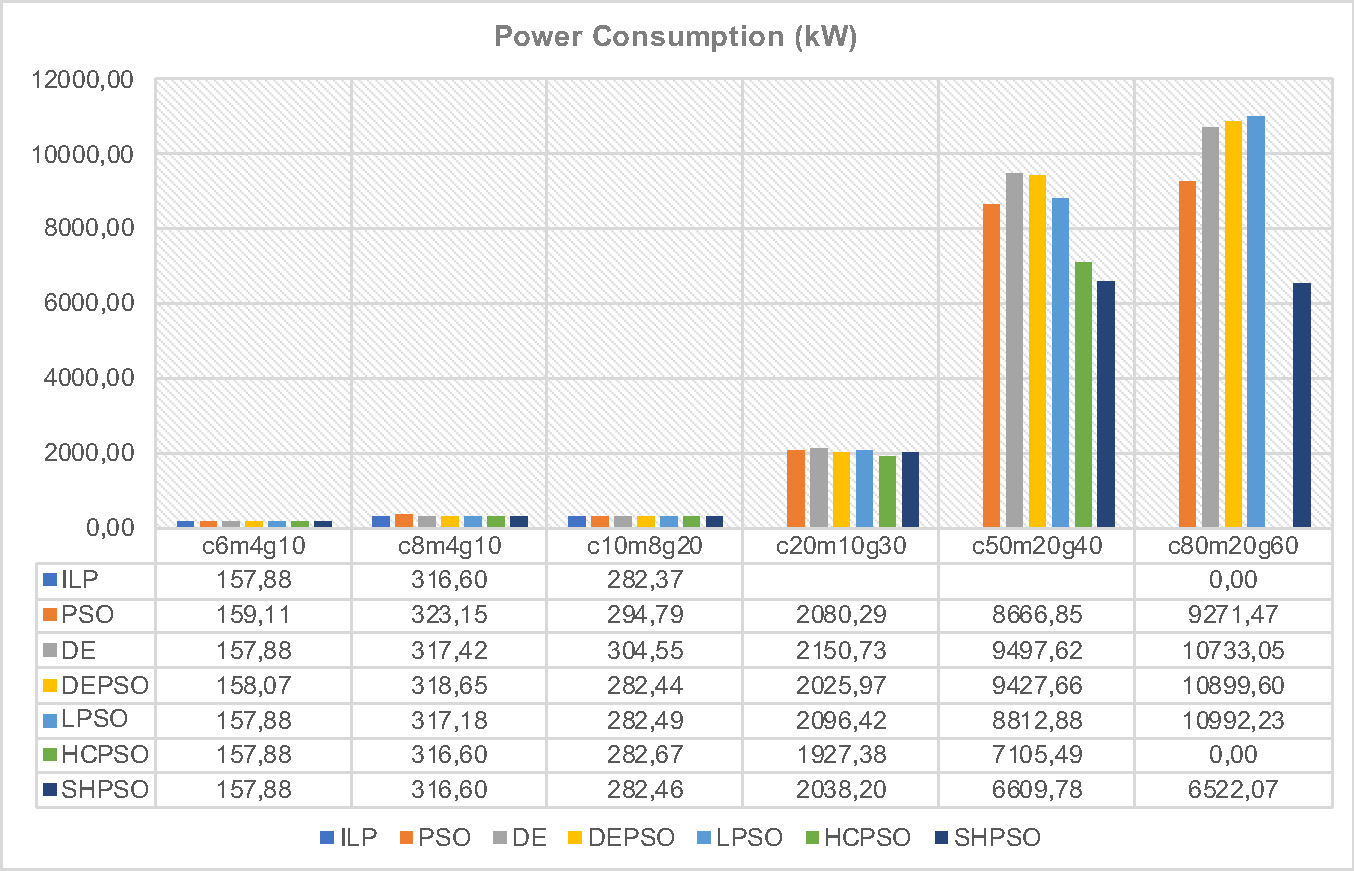
\includegraphics[width=1\linewidth]{img/power_consumption.pdf}
\caption{(Near) Optimal Power Consumption of the Different Software Allocation Problems.}
\label{fig_powerconsumption_ilp_metaheuristic}\vspace{-0.4cm}
\end{figure}

\paragraph{Convergence Time} In the case of metaheuristics, the convergence time refers to the amount of time taken by the algorithm to return solutions before the steady state where new fitness values are observed. In this evalution, it is calculated over a maximum of 5000 iterations (or generations) only for the duration before steady period, which is bounded by 5 minutes. Note: the steady time, where no fitness values change within the maximum iterations, is not considered in the converge time.  Figure \ref{fig_allocationtime_ilp_metaheuristic} summarizes the computation time of the algorithms for the samples listed in Table~\ref{tbl_fitness_allocationtime_ilp_plus_metaheuristic}. For the samples the ILP method returned solutions, the computation times are usually larger than the rest, which are in milliseconds for the $1^{st}$ sample and in seconds for the $2^{st}$  and $3^{rd}$.  The the meta-heuristic algorithms, the convergence time is in milliseconds for the first four samples, and is in seconds for the rest. However, the computation times of the meta-heuristic algorithms, which are not shown in the table usually took less than 50 minutes for the larest sample.
\begin{figure}
\centering
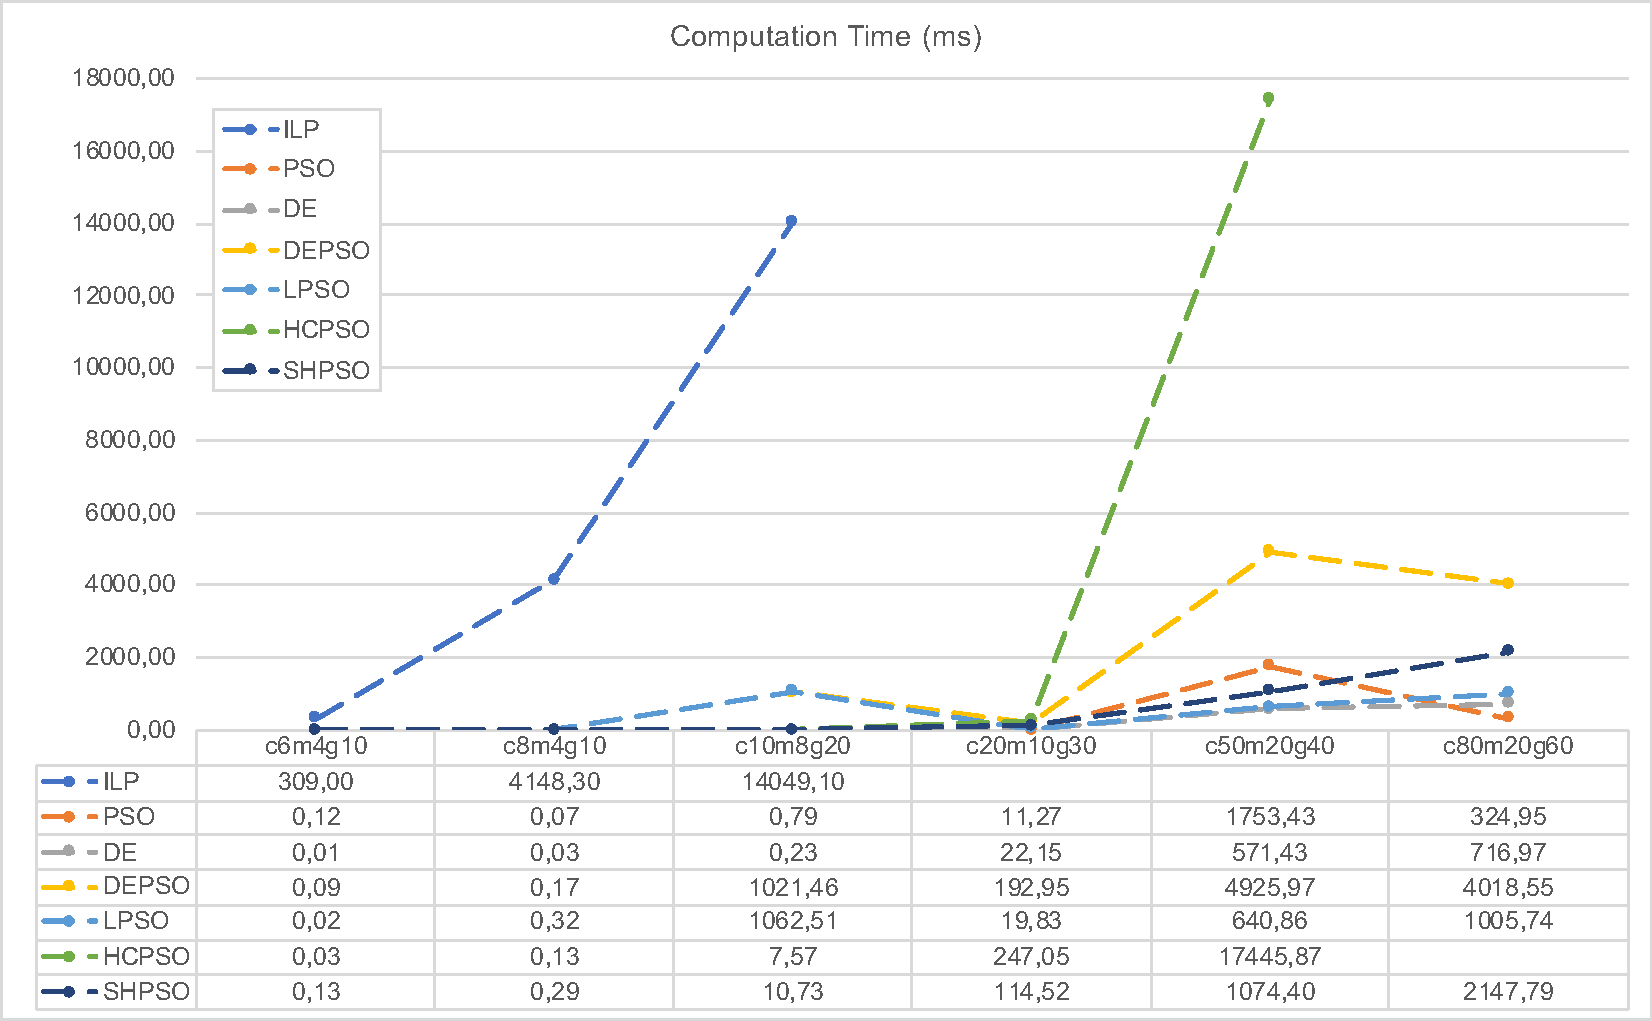
\includegraphics[width=1\linewidth]{img/time_summary.pdf}
\caption{Computation Time of the Various Algorithms for Solving Different Instances of the Software Allocation Problem.}
\label{fig_allocationtime_ilp_metaheuristic}\vspace{-0.4cm}
\end{figure}
%\begin{adjustbox}{angle=90}
\small
% Please add the following required packages to your document preamble:
% \usepackage{booktabs}

\begin{tabular}{@{}llllllllll@{}}
\toprule
Application & method & Fitness &  &  &  & power &  &  &  \\ \midrule
 &  & min & max & avg & std & min & max & avg & std \\
c6, m4,g10 & ILP & 2.28E+02 & 2.28E+02 & 2.28E+02 & 0.00E+00 & 1.58E+02 & 1.58E+02 & 1.58E+02 & 3.00E-14 \\
 & PSO & 2.28E+02 & 2.35E+02 & 2.29E+02 & 2.38E+00 & 1.58E+02 & 1.65E+02 & 1.59E+02 & 2.38E+00 \\
 & DE & 2.28E+02 & 2.28E+02 & 2.28E+02 & 3.00E-14 & 1.58E+02 & 1.58E+02 & 1.58E+02 & 3.00E-14 \\
 & DEPSO & 2.28E+02 & 2.29E+02 & 2.28E+02 & 3.08E-01 & 1.58E+02 & 1.59E+02 & 1.58E+02 & 3.09E-01 \\
 & LPSO & 2.28E+02 & 2.28E+02 & 2.28E+02 & 3.00E-14 & 1.58E+02 & 1.58E+02 & 1.58E+02 & 3.00E-14 \\
 & HCPSO & 2.28E+02 & 2.28E+02 & 2.28E+02 & 3.00E-14 & 1.58E+02 & 1.58E+02 & 1.58E+02 & 3.00E-14 \\
 & SHPSO & 2.28E+02 & 2.28E+02 & 2.28E+02 & 3.00E-14 & 1.58E+02 & 1.58E+02 & 1.58E+02 & 3.00E-14 \\
c8, m6,g20 & ILP & 4.07E+02 & 4.07E+02 & 4.07E+02 & 5.99E-14 & 3.17E+02 & 3.17E+02 & 3.17E+02 & 0.00E+00 \\
 & PSO & 4.07E+02 & 4.44E+02 & 4.15E+02 & 1.24E+01 & 3.17E+02 & 3.44E+02 & 3.23E+02 & 8.70E+00 \\
 & DE & 4.07E+02 & 4.09E+02 & 4.07E+02 & 1.05E+00 & 3.17E+02 & 3.19E+02 & 3.17E+02 & 1.05E+00 \\
 & DEPSO & 4.07E+02 & 4.35E+02 & 4.10E+02 & 8.80E+00 & 3.17E+02 & 3.35E+02 & 3.19E+02 & 5.64E+00 \\
 & LPSO & 4.07E+02 & 4.08E+02 & 4.07E+02 & 5.33E-01 & 3.17E+02 & 3.18E+02 & 3.17E+02 & 5.33E-01 \\
 & HCPSO & 4.07E+02 & 4.07E+02 & 4.07E+02 & 5.99E-14 & 3.17E+02 & 3.17E+02 & 3.17E+02 & 0.00E+00 \\
 & SHPSO & 4.07E+02 & 4.07E+02 & 4.07E+02 & 5.99E-14 & 3.17E+02 & 3.17E+02 & 3.17E+02 & 0.00E+00 \\
c10, m8,g20 & ILP & 4.42E+02 & 4.42E+02 & 4.42E+02 & 5.99E-14 & 2.82E+02 & 2.82E+02 & 2.82E+02 & 5.99E-14 \\
 & PSO & 4.42E+02 & 4.74E+02 & 4.49E+02 & 1.26E+01 & 2.82E+02 & 3.44E+02 & 2.95E+02 & 2.53E+01 \\
 & DE & 4.42E+02 & 4.97E+02 & 4.52E+02 & 1.77E+01 & 2.82E+02 & 3.67E+02 & 3.05E+02 & 3.58E+01 \\
 & DEPSO & 4.42E+02 & 4.43E+02 & 4.42E+02 & 1.90E-01 & 2.82E+02 & 2.83E+02 & 2.82E+02 & 1.90E-01 \\
 & LPSO & 4.42E+02 & 4.43E+02 & 4.42E+02 & 1.70E-01 & 2.82E+02 & 2.83E+02 & 2.82E+02 & 1.70E-01 \\
 & HCPSO & 4.42E+02 & 4.43E+02 & 4.43E+02 & 2.09E-01 & 2.82E+02 & 2.83E+02 & 2.83E+02 & 2.09E-01 \\
 & SHPSO & 4.42E+02 & 4.43E+02 & 4.42E+02 & 1.92E-01 & 2.82E+02 & 2.83E+02 & 2.82E+02 & 1.92E-01 \\
c20, m10,g30 & ILP & NA & NA & NA & NA & NA & NA & NA & NA \\
 & PSO & 5.69E+04 & 8.72E+04 & 6.46E+04 & 9.54E+03 & 1.69E+03 & 2.44E+03 & 2.08E+03 & 2.52E+02 \\
 & DE & 4.71E+04 & 6.22E+04 & 5.37E+04 & 4.13E+03 & 2.06E+03 & 2.30E+03 & 2.15E+03 & 6.56E+01 \\
 & DEPSO & 3.71E+04 & 5.22E+04 & 4.41E+04 & 4.24E+03 & 1.93E+03 & 2.17E+03 & 2.03E+03 & 8.84E+01 \\
 & LPSO & 4.73E+04 & 6.73E+04 & 5.86E+04 & 6.62E+03 & 1.66E+03 & 2.32E+03 & 2.10E+03 & 1.90E+02 \\
 & HCPSO & 4.19E+04 & 4.71E+04 & 4.25E+04 & 1.64E+03 & 1.82E+03 & 2.13E+03 & 1.93E+03 & 1.27E+02 \\
 & SHPSO & 3.73E+04 & 4.70E+04 & 4.26E+04 & 2.77E+03 & 1.93E+03 & 2.28E+03 & 2.04E+03 & 1.14E+02 \\ \bottomrule
\end{tabular}
\end{adjustbox}

\begin{adjustbox}{angle=90}
\small
% Please add the following required packages to your document preamble:
% \usepackage{booktabs}

\begin{tabular}{@{}llllllllll@{}}
\toprule
Application & method & Fitness &  &  &  & power &  &  &  \\ \midrule
 &  & min & max & avg & std & min & max & avg & std \\
c50, m20,g60 & ILP & NA & NA & NA & NA & NA & NA & NA & NA \\
 & PSO & 1.23E+06 & 1.36E+06 & 1.30E+06 & 3.86E+04 & 7.70E+03 & 9.21E+03 & 8.67E+03 & 4.78E+02 \\
 & DE & 1.39E+06 & 1.50E+06 & 1.46E+06 & 3.46E+04 & 8.67E+03 & 1.01E+04 & 9.50E+03 & 5.55E+02 \\
 & DEPSO & 1.33E+06 & 1.45E+06 & 1.38E+06 & 3.26E+04 & 8.46E+03 & 1.05E+04 & 9.43E+03 & 7.21E+02 \\
 & LPSO & 1.38E+06 & 1.48E+06 & 1.43E+06 & 3.20E+04 & 7.94E+03 & 9.90E+03 & 8.81E+03 & 6.19E+02 \\
 & HCPSO & 1.23E+06 & 1.41E+06 & 1.28E+06 & 6.53E+04 & 5.90E+03 & 7.73E+03 & 7.11E+03 & 6.41E+02 \\
 & SHPSO & 1.23E+06 & 1.41E+06 & 1.34E+06 & 9.81E+04 & 5.90E+03 & 7.32E+03 & 6.61E+03 & 1.00E+03 \\
c80, m20,g60 & ILP & NA & NA & NA & NA & NA & NA & NA & NA \\
 & PSO & 2.65E+06 & 2.74E+06 & 2.69E+06 & 4.60E+04 & 7.63E+03 & 1.06E+04 & 9.27E+03 & 1.52E+03 \\
 & DE & 2.71E+06 & 2.76E+06 & 2.74E+06 & 2.38E+04 & 8.55E+03 & 1.20E+04 & 1.07E+04 & 1.89E+03 \\
 & DEPSO & 2.55E+06 & 2.63E+06 & 2.60E+06 & 4.69E+04 & 1.01E+04 & 1.23E+04 & 1.09E+04 & 1.18E+03 \\
 & LPSO & 2.61E+06 & 2.68E+06 & 2.65E+06 & 3.58E+04 & 1.07E+04 & 1.12E+04 & 1.10E+04 & 2.50E+02 \\
 & HCPSO & NA & NA & NA & NA & NA & NA & NA & NA \\
 & SHPSO & 2.40E+06 & 2.57E+06 & 2.47E+06 & 8.94E+04 & 5.25E+03 & 7.34E+03 & 6.52E+03 & 1.12E+03 \\ \bottomrule
\end{tabular}
\end{adjustbox}
\paragraph{Solutions Stability} the PSO, DE are characterized by random search which enables exploration of higher dimenstional problems possible. However, somestime this creates instability in the solutions, that is for the same problem, it is possible to observe different performance, e.g., fitness values, computation time, etc. The stability of the solutions depend on the nature of the algorithms as well as the problems at hand. Therefore, it is crucial to evaluate the stability of the meta-heuristic algorithms used in this work. One way measuring the stability is using standar deviation, and Figure x and Figure y show the deviation of each algorithms for the (near) optimal power consumption of the different samples.

In general, with regard to quality of the solutions, the hybrid PSO with hill-climbing are more stable in the first three samples, but also DE and LPSO in $1^{st}$ sample, as compared to PSO and DEPSO. However, as the problem size increases to $1^{st},2^{nd}, 3^{rd}$,  the hybrid PSO with hill-climbing performed worse and PSO and others improved. With regard to convergence time, the stability usually decreased, that is with uniformity for the PSO, DE, HCPSO and SHPSO, however, for the rest it is not uniform.

\subsubsection{Analysis of Experiment 2}
Table~\ref{fig_chainsreplicationimprovements} shows results of executing experiment 2, which shows improvements of the computation time by applying the approximation algorithm in stead of the exact approach. In the case of the approximation, the delays are exaustively calculated in the presence of replication. However, the quality of the solutions are degraded as expected due to the approximation. Specifically, the result shown $61\%-81\%$ computation time improvement over the exac method while facing quality degradation only for samples $g_{30}d_{2}$ and  $g_{30}d_{2}$. The improvements are in seconds, which implies for a single usage (or run) of the meta-heuristic optimization algorithms, it is not significant. However, considering practical systems design process, which requires several iterations, the commulative effect of the algorithms can negatively impact the responsivess to engineers. Thus, the improvements can be in trade-off with optimality of the solutions.
\begin{figure}
	\centering
	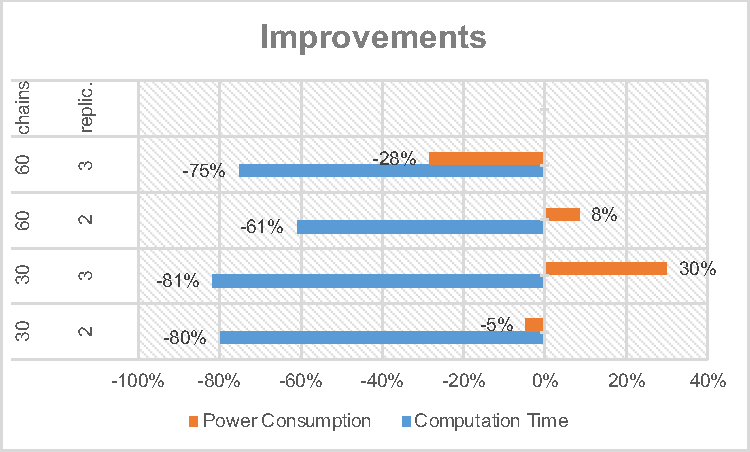
\includegraphics[width=0.7\linewidth]{img/chains_replication_improvements}
	\caption{Effect of Approximate Algorithm over Delay Calculations with Replication.}
	\label{fig_chainsreplicationimprovements}
\end{figure}

\section{Discussion}
